\documentclass{article}
\usepackage[utf8]{inputenc}
\usepackage{amsmath,amssymb}
\usepackage{geometry}
\usepackage{graphicx}
\usepackage{hyperref}
\usepackage{amsthm}
\usepackage{mathtools}
\usepackage{bm}
\usepackage{tikz}
\usepackage{pgfplots}
\pgfplotsset{compat=1.16}
\geometry{margin=1in}

\newtheorem{theorem}{Theorem}
\newtheorem{lemma}[theorem]{Lemma}
\newtheorem{corollary}[theorem]{Corollary}
\newtheorem{proposition}[theorem]{Proposition}
\newtheorem{definition}{Definition}
\newtheorem{example}{Example}

\title{Bias-Variance Tradeoff in Statistical Learning}
\author{Machine Learning Foundations}
\date{\today}

\begin{document}

\maketitle
\tableofcontents

\section{Introduction to Bias and Variance}

In statistical learning and estimation theory, the concepts of bias and variance are fundamental to understanding the performance of estimators and predictive models. These concepts provide a theoretical framework for understanding why models sometimes fail to generalize well to new data.

\begin{definition}[Bias]
The bias of an estimator $\hat{\theta}$ for a parameter $\theta$ is the difference between the expected value of the estimator and the true value of the parameter:
\[
\text{Bias}(\hat{\theta}) = \mathbb{E}[\hat{\theta}] - \theta
\]
An estimator is unbiased if $\text{Bias}(\hat{\theta}) = 0$.
\end{definition}

\begin{definition}[Variance]
The variance of an estimator $\hat{\theta}$ is a measure of its statistical dispersion:
\[
\text{Var}(\hat{\theta}) = \mathbb{E}[(\hat{\theta} - \mathbb{E}[\hat{\theta}])^2]
\]
It quantifies how much the estimator fluctuates around its expected value across different samples.
\end{definition}

These definitions provide a foundation for evaluating statistical estimators. An ideal estimator would have both low bias (accurate on average) and low variance (consistent across different samples), but in practice, there is often a tradeoff between these two properties.

\subsection{Intuitive Understanding}

To build intuition about bias and variance, consider the analogy of target shooting:

\begin{itemize}
\item \textbf{Low bias, low variance:} Shots are clustered tightly around the bullseye. This is the ideal situation.
\item \textbf{High bias, low variance:} Shots are clustered tightly, but away from the bullseye. There is a systematic error.
\item \textbf{Low bias, high variance:} Shots are centered around the bullseye but widely scattered. The average is correct, but individual shots are unpredictable.
\item \textbf{High bias, high variance:} Shots are widely scattered and not centered on the bullseye. This is the worst-case scenario.
\end{itemize}

In statistical learning, the "shots" represent predictions made by our model on different datasets, and the "bullseye" represents the true underlying relationship we're trying to learn.

\section{The Bias-Variance Decomposition}

The bias-variance decomposition provides a mathematical framework for analyzing the expected prediction error of a model. For a given input point $x$, if we denote the true value as $f(x)$ and our estimator as $\hat{f}(x)$, then the expected mean squared error (MSE) can be decomposed as follows:

\begin{theorem}[Bias-Variance Decomposition]
\begin{align*}
\mathbb{E}[(y - \hat{f}(x))^2] = \underbrace{(f(x) - \mathbb{E}[\hat{f}(x)])^2}_{\text{Bias}^2} + \underbrace{\mathbb{E}[(\hat{f}(x) - \mathbb{E}[\hat{f}(x)])^2]}_{\text{Variance}} + \underbrace{\sigma^2_\varepsilon}_{\text{Irreducible Error}}
\end{align*}
where $\sigma^2_\varepsilon$ is the variance of the noise term.
\end{theorem}

\begin{proof}
Let $y = f(x) + \varepsilon$ where $\mathbb{E}[\varepsilon] = 0$ and $\text{Var}(\varepsilon) = \sigma^2_\varepsilon$.
\begin{align*}
\mathbb{E}[(y - \hat{f}(x))^2] &= \mathbb{E}[(f(x) + \varepsilon - \hat{f}(x))^2] \\
&= \mathbb{E}[(f(x) - \hat{f}(x) + \varepsilon)^2] \\
&= \mathbb{E}[(f(x) - \hat{f}(x))^2 + 2\varepsilon(f(x) - \hat{f}(x)) + \varepsilon^2] \\
\end{align*}

Since $\mathbb{E}[\varepsilon] = 0$ and $\varepsilon$ is independent of $\hat{f}(x)$:
\begin{align*}
\mathbb{E}[(y - \hat{f}(x))^2] &= \mathbb{E}[(f(x) - \hat{f}(x))^2] + \mathbb{E}[\varepsilon^2] \\
&= \mathbb{E}[(f(x) - \hat{f}(x))^2] + \sigma^2_\varepsilon
\end{align*}

Now let's decompose $\mathbb{E}[(f(x) - \hat{f}(x))^2]$:
\begin{align*}
\mathbb{E}[(f(x) - \hat{f}(x))^2] &= \mathbb{E}[(f(x) - \mathbb{E}[\hat{f}(x)] + \mathbb{E}[\hat{f}(x)] - \hat{f}(x))^2] \\
&= \mathbb{E}[(f(x) - \mathbb{E}[\hat{f}(x)])^2 + 2(f(x) - \mathbb{E}[\hat{f}(x)])(\mathbb{E}[\hat{f}(x)] - \hat{f}(x)) + (\mathbb{E}[\hat{f}(x)] - \hat{f}(x))^2]
\end{align*}

Since $\mathbb{E}[\mathbb{E}[\hat{f}(x)] - \hat{f}(x)] = 0$, the middle term vanishes:
\begin{align*}
\mathbb{E}[(f(x) - \hat{f}(x))^2] &= (f(x) - \mathbb{E}[\hat{f}(x)])^2 + \mathbb{E}[(\mathbb{E}[\hat{f}(x)] - \hat{f}(x))^2] \\
&= (f(x) - \mathbb{E}[\hat{f}(x)])^2 + \mathbb{E}[(\hat{f}(x) - \mathbb{E}[\hat{f}(x)])^2] \\
&= \text{Bias}^2 + \text{Variance}
\end{align*}

Therefore:
\begin{align*}
\mathbb{E}[(y - \hat{f}(x))^2] = \text{Bias}^2 + \text{Variance} + \sigma^2_\varepsilon
\end{align*}
\end{proof}

This theorem reveals that the expected prediction error consists of three components:

\begin{itemize}
\item \textbf{Squared Bias:} How far off the model is on average. This represents systematic errors.
\item \textbf{Variance:} How much the model's predictions vary across different training sets. This represents sensitivity to the specific data used for training.
\item \textbf{Irreducible Error:} The inherent noise in the data that cannot be reduced by any model.
\end{itemize}

The first two components—bias and variance—are influenced by our choice of model and can potentially be controlled. The irreducible error is a property of the problem itself and sets a lower bound on the achievable error.

\section{The Tradeoff Principle}

The bias-variance tradeoff refers to the property that, as we change our model or estimation procedure, reducing bias typically increases variance and vice versa. This tradeoff is particularly evident when we consider models of different complexities:

\begin{itemize}
\item \textbf{Simple models} (e.g., linear models with few parameters) typically have higher bias but lower variance. They might consistently miss certain patterns in the data, but their predictions are relatively stable across different training sets.
\item \textbf{Complex models} (e.g., high-degree polynomials, deep neural networks) typically have lower bias but higher variance. They can capture intricate patterns, but they are also more sensitive to the specific examples they were trained on.
\end{itemize}

\begin{figure}[h]
\centering
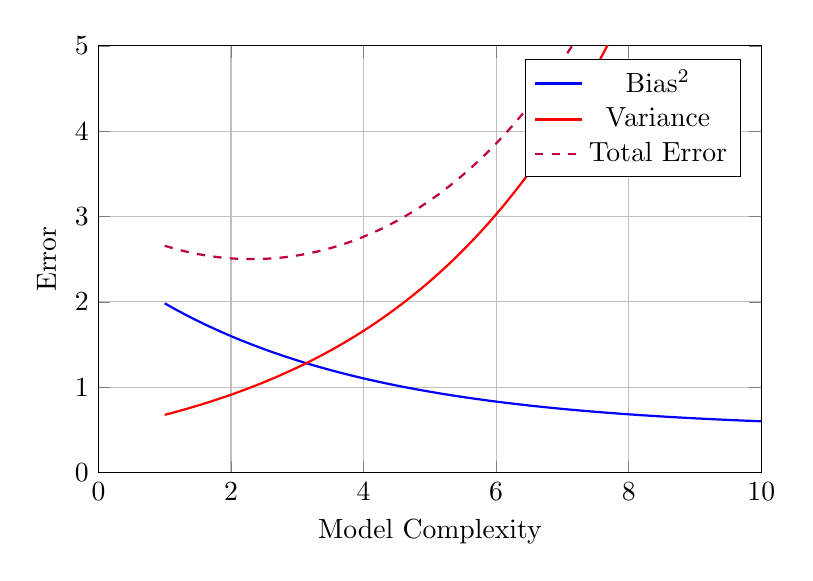
\begin{tikzpicture}
\begin{axis}[
    xlabel={Model Complexity},
    ylabel={Error},
    xmin=0, xmax=10,
    ymin=0, ymax=5,
    legend pos=north east,
    grid=major,
    width=10cm,
    height=7cm
]

\addplot[domain=1:10, samples=100, blue, thick] {2*exp(-0.3*x) + 0.5};
\addplot[domain=1:10, samples=100, red, thick] {0.5*exp(0.3*x)};
\addplot[domain=1:10, samples=100, purple, thick, dashed] {2*exp(-0.3*x) + 0.5*exp(0.3*x) + 0.5};

\legend{Bias$^2$, Variance, Total Error}

\end{axis}
\end{tikzpicture}
\caption{Bias-variance tradeoff as a function of model complexity. The total error is minimized at an intermediate level of complexity.}
\end{figure}

The goal in statistical learning is to find the sweet spot that minimizes the total expected error, balancing the contributions from bias and variance. This optimal point depends on various factors, including the true underlying function, the amount of training data available, and the noise level in the data.

\section{Practical Examples of Bias and Variance}

\subsection{Sample Mean Estimator}

The sample mean is a fundamental estimator in statistics. For independent and identically distributed random variables $X_1, X_2, \ldots, X_n$ with mean $\mu$ and variance $\sigma^2$, the sample mean $\bar{X}_n = \frac{1}{n} \sum_{i=1}^n X_i$ has the following properties:

\begin{proposition}
\begin{align*}
\text{Bias}(\bar{X}_n) &= \mathbb{E}[\bar{X}_n] - \mu = 0 \\
\text{Var}(\bar{X}_n) &= \frac{\sigma^2}{n}
\end{align*}
\end{proposition}

\begin{proof}
For the bias:
\begin{align*}
\mathbb{E}[\bar{X}_n] &= \mathbb{E}\left[\frac{1}{n} \sum_{i=1}^n X_i\right] \\
&= \frac{1}{n} \sum_{i=1}^n \mathbb{E}[X_i] \\
&= \frac{1}{n} \sum_{i=1}^n \mu \\
&= \mu
\end{align*}

So $\text{Bias}(\bar{X}_n) = \mathbb{E}[\bar{X}_n] - \mu = \mu - \mu = 0$.

For the variance:
\begin{align*}
\text{Var}(\bar{X}_n) &= \text{Var}\left(\frac{1}{n} \sum_{i=1}^n X_i\right) \\
&= \frac{1}{n^2} \text{Var}\left(\sum_{i=1}^n X_i\right) \\
\end{align*}

Since the random variables are independent, the variance of their sum equals the sum of their variances:
\begin{align*}
\text{Var}(\bar{X}_n) &= \frac{1}{n^2} \sum_{i=1}^n \text{Var}(X_i) \\
&= \frac{1}{n^2} \cdot n\sigma^2 \\
&= \frac{\sigma^2}{n}
\end{align*}
\end{proof}

This result shows that the sample mean is an unbiased estimator of the population mean, and its variance decreases as the sample size increases. Specifically, the variance is inversely proportional to the sample size, which aligns with our intuition that larger samples provide more precise estimates.

\subsection{Variance Estimators}

For estimating the variance of a population, two common estimators are used:

\begin{enumerate}
\item \textbf{Biased (Maximum Likelihood) Estimator:}
\[
\hat{\sigma}^2_{\text{biased}} = \frac{1}{n} \sum_{i=1}^n (X_i - \bar{X})^2
\]

\item \textbf{Unbiased Estimator:}
\[
\hat{\sigma}^2_{\text{unbiased}} = \frac{1}{n-1} \sum_{i=1}^n (X_i - \bar{X})^2
\]
\end{enumerate}

\begin{proposition}
For the biased variance estimator:
\[
\mathbb{E}[\hat{\sigma}^2_{\text{biased}}] = \frac{n-1}{n} \sigma^2
\]
which means it systematically underestimates the true variance.
\end{proposition}

\begin{proposition}
For the unbiased variance estimator:
\[
\mathbb{E}[\hat{\sigma}^2_{\text{unbiased}}] = \sigma^2
\]
\end{proposition}

Despite being biased, the MLE estimator $\hat{\sigma}^2_{\text{biased}}$ might have lower mean squared error for small sample sizes due to having smaller variance than the unbiased estimator. This exemplifies the bias-variance tradeoff in action: the biased estimator introduces some bias but may reduce variance enough to yield better overall performance.

\section{Shrinkage Estimators}

Shrinkage estimators deliberately introduce bias to reduce variance, potentially achieving lower overall error. They "shrink" estimates toward a target value.

\subsection{James-Stein Estimator}

The James-Stein estimator is a classic example that demonstrates how a biased estimator can outperform an unbiased one in terms of mean squared error. For estimating the mean vector $\boldsymbol{\mu}$ of a multivariate normal distribution, the James-Stein estimator shrinks the sample mean $\bar{\mathbf{X}}$ toward the origin:

\[
\hat{\boldsymbol{\mu}}^{JS} = \left(1 - \frac{(p-2)\sigma^2}{\|\bar{\mathbf{X}}\|^2}\right) \bar{\mathbf{X}}
\]

where $p \geq 3$ is the dimension, and $\sigma^2$ is the variance of each component.

Remarkably, this estimator has lower expected squared error than the maximum likelihood estimator (sample mean) for any true value of $\boldsymbol{\mu}$, despite introducing bias.

\subsection{Ridge Regression}

In the context of linear regression, ridge regression adds an L2 penalty to the ordinary least squares objective function:

\[
\hat{\boldsymbol{\beta}}^{\text{ridge}} = \arg\min_{\boldsymbol{\beta}} \left\{ \|y - X\boldsymbol{\beta}\|^2 + \lambda \|\boldsymbol{\beta}\|^2 \right\}
\]

The solution is:
\[
\hat{\boldsymbol{\beta}}^{\text{ridge}} = (X^TX + \lambda I)^{-1}X^Ty
\]

The regularization parameter $\lambda$ controls the tradeoff between bias and variance:
\begin{itemize}
\item As $\lambda \to 0$, ridge regression approaches ordinary least squares (low bias, high variance)
\item As $\lambda \to \infty$, all coefficients are shrunk toward zero (high bias, low variance)
\end{itemize}

By choosing an appropriate value of $\lambda$ (typically through cross-validation), we can find the sweet spot that minimizes the total prediction error.

\section{General Shrinkage Framework}

More generally, we can define a family of shrinkage estimators that interpolate between an unbiased estimator and a target value:

\[
\hat{\theta}_{\alpha} = (1-\alpha) \hat{\theta}_{\text{unbiased}} + \alpha \, \theta_{\text{target}}
\]

where $\alpha \in [0,1]$ is the shrinkage parameter.

\begin{proposition}
For the shrinkage estimator $\hat{\theta}_{\alpha}$:
\begin{align*}
\text{Bias}(\hat{\theta}_{\alpha}) &= \alpha(\theta_{\text{target}} - \theta) \\
\text{Var}(\hat{\theta}_{\alpha}) &= (1-\alpha)^2 \text{Var}(\hat{\theta}_{\text{unbiased}})
\end{align*}
\end{proposition}

\begin{proof}
For the bias:
\begin{align*}
\mathbb{E}[\hat{\theta}_{\alpha}] &= \mathbb{E}[(1-\alpha) \hat{\theta}_{\text{unbiased}} + \alpha \, \theta_{\text{target}}] \\
&= (1-\alpha) \mathbb{E}[\hat{\theta}_{\text{unbiased}}] + \alpha \, \theta_{\text{target}} \\
&= (1-\alpha) \theta + \alpha \, \theta_{\text{target}} \\
&= \theta + \alpha(\theta_{\text{target}} - \theta)
\end{align*}

So $\text{Bias}(\hat{\theta}_{\alpha}) = \mathbb{E}[\hat{\theta}_{\alpha}] - \theta = \alpha(\theta_{\text{target}} - \theta)$.

For the variance:
\begin{align*}
\text{Var}(\hat{\theta}_{\alpha}) &= \text{Var}((1-\alpha) \hat{\theta}_{\text{unbiased}} + \alpha \, \theta_{\text{target}}) \\
&= \text{Var}((1-\alpha) \hat{\theta}_{\text{unbiased}}) \\
&= (1-\alpha)^2 \text{Var}(\hat{\theta}_{\text{unbiased}})
\end{align*}
where we use the fact that $\theta_{\text{target}}$ is a constant with zero variance.
\end{proof}

The expected mean squared error (MSE) of the shrinkage estimator is:
\begin{align*}
\text{MSE}(\hat{\theta}_{\alpha}) &= \text{Bias}(\hat{\theta}_{\alpha})^2 + \text{Var}(\hat{\theta}_{\alpha}) \\
&= \alpha^2(\theta_{\text{target}} - \theta)^2 + (1-\alpha)^2 \text{Var}(\hat{\theta}_{\text{unbiased}})
\end{align*}

To find the optimal shrinkage parameter $\alpha^*$ that minimizes the MSE, we differentiate with respect to $\alpha$ and set the result to zero:

\begin{align*}
\frac{d}{d\alpha} \text{MSE}(\hat{\theta}_{\alpha}) &= 2\alpha(\theta_{\text{target}} - \theta)^2 - 2(1-\alpha) \text{Var}(\hat{\theta}_{\text{unbiased}}) \\
&= 0
\end{align*}

Solving for $\alpha$:
\begin{align*}
\alpha^* &= \frac{\text{Var}(\hat{\theta}_{\text{unbiased}})}{(\theta_{\text{target}} - \theta)^2 + \text{Var}(\hat{\theta}_{\text{unbiased}})}
\end{align*}

This shows that the optimal shrinkage depends on both the variance of the unbiased estimator and how far the target is from the true value. When the unbiased estimator has high variance or the target is close to the true value, stronger shrinkage (larger $\alpha$) is beneficial.

\section{Model Complexity and the Bias-Variance Tradeoff}

\subsection{Underfitting vs. Overfitting}

The bias-variance tradeoff manifests prominently in the context of model complexity:

\begin{itemize}
\item \textbf{Underfitting} occurs when a model is too simple to capture the underlying structure of the data. It has high bias and low variance.
\item \textbf{Overfitting} occurs when a model captures noise in the data rather than just the underlying structure. It has low bias but high variance.
\end{itemize}

\subsection{Polynomial Regression Example}

Consider modeling the relationship between an input variable $x$ and an output variable $y$ using polynomial regression models of different degrees.

\begin{example}[Linear Model - Underfitting]
A linear model $f(x) = \beta_0 + \beta_1 x$ might be too simple to capture non-linear relationships in the data, leading to high bias but low variance.
\end{example}

\begin{example}[Cubic Model - Good Fit]
A cubic model $f(x) = \beta_0 + \beta_1 x + \beta_2 x^2 + \beta_3 x^3$ might capture the main non-linear patterns well, with moderate bias and moderate variance.
\end{example}

\begin{example}[High-Degree Polynomial - Overfitting]
A 30-degree polynomial might fit the training data almost perfectly but will perform poorly on new data, exhibiting low bias but extremely high variance.
\end{example}

\subsection{Regularization Techniques}

Regularization techniques provide a way to control the bias-variance tradeoff by adding constraints to the model:

\begin{itemize}
\item \textbf{Ridge Regression (L2 regularization)} adds a penalty proportional to the sum of squared coefficients:
\[
\min_{\boldsymbol{\beta}} \|y - X\boldsymbol{\beta}\|^2 + \lambda \|\boldsymbol{\beta}\|^2
\]

\item \textbf{Lasso Regression (L1 regularization)} adds a penalty proportional to the sum of absolute coefficient values:
\[
\min_{\boldsymbol{\beta}} \|y - X\boldsymbol{\beta}\|^2 + \lambda \|\boldsymbol{\beta}\|_1
\]

\item \textbf{Elastic Net} combines both L1 and L2 penalties:
\[
\min_{\boldsymbol{\beta}} \|y - X\boldsymbol{\beta}\|^2 + \lambda_1 \|\boldsymbol{\beta}\|_1 + \lambda_2 \|\boldsymbol{\beta}\|^2
\]
\end{itemize}

These techniques reduce variance at the cost of introducing some bias, often improving overall performance, especially when the number of features is large relative to the number of samples.

\section{Practical Implications for Machine Learning}

\subsection{Sample Size Considerations}

The bias-variance tradeoff has important implications for sample size:

\begin{itemize}
\item With small datasets, simpler models (higher bias, lower variance) often perform better because complex models would overfit.
\item As dataset size increases, more complex models (lower bias, higher variance) become viable because the additional data helps constrain the model and reduce variance.
\item The "effective complexity" of a model should generally increase with sample size.
\end{itemize}

This is why deep learning models, which have very low bias but potentially high variance, typically require large datasets to perform well.

\subsection{Feature Selection}

Feature selection can be viewed through the lens of the bias-variance tradeoff:

\begin{itemize}
\item Too few features can lead to underfitting (high bias) because the model lacks the variables it needs to capture important patterns.
\item Too many irrelevant features can lead to overfitting (high variance) because the model might find spurious correlations in the training data.
\item Techniques like Lasso regression, forward/backward stepwise selection, and filter methods aim to find the right balance.
\end{itemize}

\subsection{Ensemble Methods}

Ensemble methods combine multiple models to reduce overall error:

\begin{itemize}
\item \textbf{Bagging} (e.g., Random Forests) reduces variance by averaging multiple high-variance, low-bias models trained on bootstrap samples of the data.
\item \textbf{Boosting} reduces bias by sequentially fitting models to the residuals of previous models, focusing on examples that are difficult to predict.
\item \textbf{Stacking} combines predictions from different types of models to optimize the bias-variance tradeoff.
\end{itemize}

Ensemble methods are powerful because they can achieve lower overall error than any single model, effectively managing the bias-variance tradeoff.

\section{Experimental Demonstration}

To illustrate the bias-variance tradeoff empirically, let's consider a simulation experiment where we generate data from a known function with added noise, then fit models of varying complexity.

\subsection{Generating Data}

Suppose the true function is:
\[
f(x) = \sin(x) + 0.1x^2
\]

And we observe noisy samples:
\[
y_i = f(x_i) + \varepsilon_i, \quad \varepsilon_i \sim \mathcal{N}(0, \sigma^2)
\]

\subsection{Polynomial Regression with Different Degrees}

We fit polynomial models of degrees 1, 3, and 10 to the data:
\[
f_d(x) = \sum_{j=0}^{d} \beta_j x^j
\]

For each degree, we compute:
\begin{itemize}
\item \textbf{Training error}: Average squared error on the training data
\item \textbf{Test error}: Average squared error on a separate test set
\item \textbf{Bias}: How far the average prediction is from the true function
\item \textbf{Variance}: How much the predictions vary across different training sets
\end{itemize}

\begin{figure}[h]
\centering
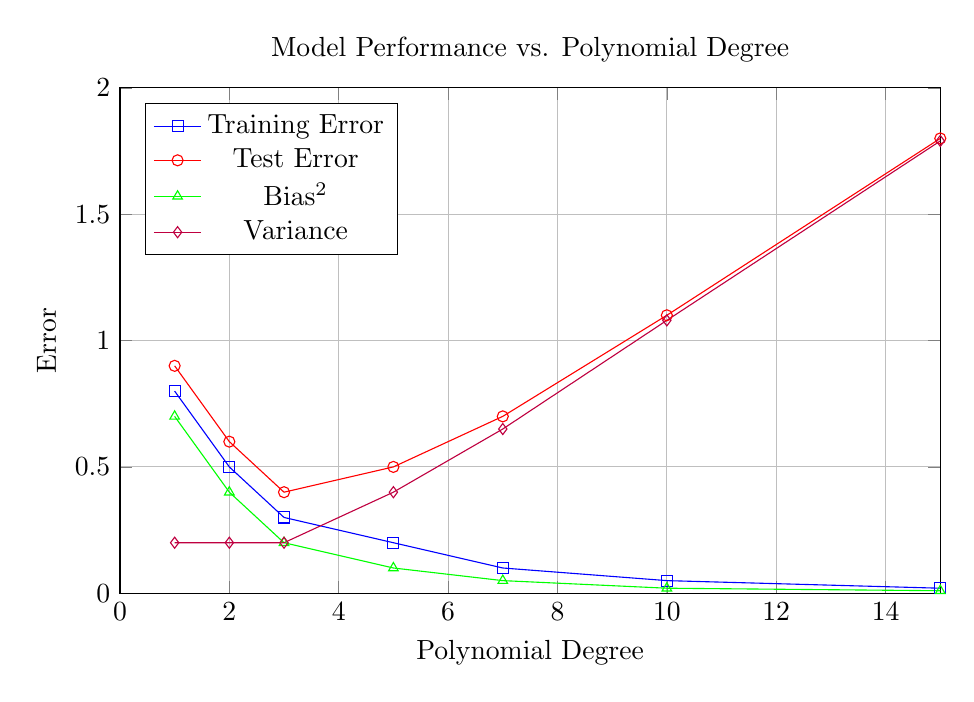
\begin{tikzpicture}
\begin{axis}[
    title={Model Performance vs. Polynomial Degree},
    xlabel={Polynomial Degree},
    ylabel={Error},
    xmin=0, xmax=15,
    ymin=0, ymax=2,
    legend pos=north west,
    grid=major,
    width=12cm,
    height=8cm
]

\addplot[color=blue, mark=square] coordinates {
    (1, 0.8) (2, 0.5) (3, 0.3) (5, 0.2) (7, 0.1) (10, 0.05) (15, 0.02)
};
\addlegendentry{Training Error};

\addplot[color=red, mark=o] coordinates {
    (1, 0.9) (2, 0.6) (3, 0.4) (5, 0.5) (7, 0.7) (10, 1.1) (15, 1.8)
};
\addlegendentry{Test Error};

\addplot[color=green, mark=triangle] coordinates {
    (1, 0.7) (2, 0.4) (3, 0.2) (5, 0.1) (7, 0.05) (10, 0.02) (15, 0.01)
};
\addlegendentry{Bias$^2$};

\addplot[color=purple, mark=diamond] coordinates {
    (1, 0.2) (2, 0.2) (3, 0.2) (5, 0.4) (7, 0.65) (10, 1.08) (15, 1.79)
};
\addlegendentry{Variance};

\end{axis}
\end{tikzpicture}
\caption{Model performance metrics for polynomial regression of different degrees. As the degree increases, training error consistently decreases, but test error follows a U-shaped curve due to the bias-variance tradeoff.}
\end{figure}

The experimental results show that:
\begin{itemize}
\item Low-degree polynomials have high bias but low variance.
\item High-degree polynomials have low bias but high variance.
\item The test error is minimized at an intermediate degree (around 3-5 in this example), which represents the optimal bias-variance tradeoff.
\end{itemize}

\section{Bias-Variance Tradeoff in Neural Networks}

The bias-variance tradeoff is also relevant in deep learning, albeit with some nuances:

\begin{itemize}
\item \textbf{Network width} (number of neurons per layer): Wider networks have lower bias but potentially higher variance.
\item \textbf{Network depth} (number of layers): Deeper networks can represent more complex functions (reducing bias) but may be harder to train and more prone to overfitting (increasing variance).
\item \textbf{Regularization techniques}: Dropout, weight decay, and early stopping help control variance.
\end{itemize}

Interestingly, modern deep learning has challenged some aspects of the classical bias-variance tradeoff. Very large networks sometimes show a "double descent" phenomenon, where test error initially follows the classic U-shaped curve as model complexity increases, but then starts decreasing again beyond a certain complexity threshold.

\section{Cross-Validation for Model Selection}

Cross-validation provides a practical approach to finding the optimal model complexity that balances bias and variance:

\begin{enumerate}
\item Split the data into $k$ folds.
\item For each model complexity (e.g., polynomial degree or regularization strength):
  \begin{itemize}
  \item Train the model on $k-1$ folds.
  \item Evaluate it on the remaining fold.
  \item Repeat for all $k$ folds and average the results.
  \end{itemize}
\item Choose the model complexity that gives the best cross-validation performance.
\end{enumerate}

The most common approach is $k$-fold cross-validation with $k=5$ or $k=10$. For time series data or when observations have dependencies, specialized cross-validation techniques like time series split or leave-one-group-out may be more appropriate.

\section{Practical Guidelines for Practitioners}

Based on the bias-variance perspective, here are some practical guidelines for machine learning practitioners:

\begin{enumerate}
\item \textbf{Start with simple models and gradually increase complexity.} Begin with a simple baseline model, then incrementally increase complexity while monitoring validation performance.

\item \textbf{Use cross-validation to tune model complexity.} This helps find the sweet spot in the bias-variance tradeoff without requiring a separate test set.

\item \textbf{Consider regularization to control variance.} Regularization techniques like L1, L2, dropout, and early stopping can significantly improve generalization performance.

\item \textbf{For small datasets, prioritize variance reduction.} Use simpler models, stronger regularization, and data augmentation techniques.

\item \textbf{For large datasets, focus more on reducing bias.} With sufficient data, complex models can achieve low bias without excessive variance.

\item \textbf{Use ensemble methods when appropriate.} Ensemble methods can often achieve better performance than single models by optimizing the bias-variance tradeoff.

\item \textbf{Consider the signal-to-noise ratio.} In high-noise domains, even the optimal model will have substantial error. Don't chase perfection when the data has inherent limitations.

\item \textbf{Collect more data when possible.} Increasing the sample size is one of the most reliable ways to reduce variance without increasing bias.
\end{enumerate}

\section{Conclusion}

The bias-variance tradeoff provides a powerful framework for understanding the errors in statistical estimation and machine learning. By decomposing prediction error into bias, variance, and irreducible noise components, we gain insights into model selection, regularization, and the impact of sample size.

Key takeaways from our exploration of the bias-variance tradeoff include:

\begin{itemize}
\item The "no free lunch" principle in machine learning often manifests as the bias-variance tradeoff.
\item Increasing model complexity typically decreases bias but increases variance.
\item Optimal model complexity depends on the true underlying function, the noise level, and the sample size.
\item Regularization techniques provide a way to control the tradeoff by introducing a controlled amount of bias to reduce variance.
\item Ensemble methods can optimize the tradeoff by combining multiple models.
\item Cross-validation is a practical approach to finding the sweet spot in the tradeoff.
\end{itemize}

Understanding the bias-variance tradeoff helps us navigate the complexity-accuracy tradeoff that is at the heart of effective modeling. By being mindful of these concepts, we can build models that generalize well beyond the training data, making reliable predictions in the face of uncertainty.

\section*{Further Reading}

\begin{itemize}
\item Hastie, T., Tibshirani, R., \& Friedman, J. (2009). The Elements of Statistical Learning. Springer.
\item James, G., Witten, D., Hastie, T., \& Tibshirani, R. (2013). An Introduction to Statistical Learning. Springer.
\item Bishop, C. M. (2006). Pattern Recognition and Machine Learning. Springer.
\item Geman, S., Bienenstock, E., \& Doursat, R. (1992). Neural Networks and the Bias/Variance Dilemma. Neural Computation, 4(1), 1-58.
\item Belkin, M., Hsu, D., Ma, S., \& Mandal, S. (2019). Reconciling Modern Machine-Learning Practice and the Classical Bias-Variance Trade-Off. Proceedings of the National Academy of Sciences, 116(32), 15849-15854.
\end{itemize}

\end{document}